% Original teaching adaptation of Heather Macbeth, The Mechanics of Proof, Chapter 10.
% Source: https://hrmacbeth.github.io/math2001/10_Relations.html
% Source repository: hrmacbeth/math2001, e660f42b13ddcb6d12b52ba036d6bd071a0cfb9b.
% Prose, solution organization, and TikZ drawings are new. Lean listings are not build-verified.
% CSC302 lecture slides adapted from Heather Macbeth, The Mechanics of Proof.
\documentclass[aspectratio=169,11pt]{beamer}
\usepackage[T1]{fontenc}
\usepackage{lmodern}
\usepackage{amsmath,amssymb,mathtools}
\usepackage{booktabs,array,listings,tikz}
\usetikzlibrary{arrows.meta,positioning,calc}
\definecolor{ProofNavy}{HTML}{18324F}
\definecolor{ProofTeal}{HTML}{007D82}
\definecolor{ProofPaper}{HTML}{F3F6F8}
\usetheme{default}
\setbeamercolor{normal text}{fg=ProofNavy,bg=white}
\setbeamercolor{structure}{fg=ProofTeal}
\setbeamercolor{frametitle}{fg=ProofNavy}
\setbeamercolor{block title}{fg=white,bg=ProofNavy}
\setbeamercolor{block body}{fg=ProofNavy,bg=ProofPaper}
\setbeamercolor{block title example}{fg=white,bg=ProofTeal}
\setbeamercolor{block body example}{fg=ProofNavy,bg=ProofPaper}
\setbeamerfont{frametitle}{size=\Large,series=\bfseries}
\setbeamertemplate{navigation symbols}{}
\setbeamertemplate{itemize item}{\small\textbullet}
\setbeamertemplate{footline}{%
  \leavevmode\hbox{%
  \begin{beamercolorbox}[wd=.86\paperwidth,ht=2.8ex,dp=1.2ex,leftskip=1.6em]{author in head/foot}%
    \scriptsize CSC302\quad\textbar\quad\insertshorttitle
  \end{beamercolorbox}%
  \begin{beamercolorbox}[wd=.14\paperwidth,ht=2.8ex,dp=1.2ex,rightskip=1.6em plus1fil]{date in head/foot}%
    \scriptsize\insertframenumber/\inserttotalframenumber
  \end{beamercolorbox}}}
\setbeamersize{text margin left=8mm,text margin right=8mm}
\lstdefinelanguage{Lean}{%
  morekeywords={example,theorem,lemma,def,by,calc,have,exact,apply,intro,intros,constructor,rcases,rfl,rw,ring,numbers,linarith,nlinarith,rel,extra,addarith,obtain,left,right,use,choose,dsimp,change,ext,fun,show,from,at,with,induction,case,decide,contradiction,push_neg,by_cases,by_contra,assumption,existsi,simp,simpa},
  sensitive=true,morecomment=[l]{--},morestring=[b]"}
\lstset{language=Lean,basicstyle=\ttfamily\small,keywordstyle=\color{ProofTeal}\bfseries,
  commentstyle=\color{gray},stringstyle=\color{ProofNavy},showstringspaces=false,
  columns=fullflexible,keepspaces=true,breaklines=true,frame=single,
  rulecolor=\color{ProofTeal!30},backgroundcolor=\color{ProofPaper},
  aboveskip=0.5em,belowskip=0.4em}
\newcommand{\N}{\mathbb{N}}
\newcommand{\Z}{\mathbb{Z}}
\newcommand{\Q}{\mathbb{Q}}
\newcommand{\R}{\mathbb{R}}
\newcommand{\coursechapter}[2]{%
  \title[Chapter #1: #2]{Chapter #1\\#2}%
  \subtitle{The Mechanics of Proof \textbar{} CSC302 lecture notes}%
  \author{Based on Heather Macbeth's textbook}%
  \date{}%
}
\newcommand{\sourcecredit}[1]{\par\vfill{\tiny Source: Heather Macbeth, \emph{The Mechanics of Proof}, #1.}}
\newcommand{\bookurl}{\url{https://hrmacbeth.github.io/math2001/}}
\hypersetup{colorlinks=true,urlcolor=ProofTeal,linkcolor=ProofNavy}

\coursechapter{10}{Relations}
\begin{document}
\begin{frame}
\titlepage
\end{frame}

% Source: Chapter 10 introduction and the two section headings.
\begin{frame}{What we will learn}
\begin{itemize}
\item Test reflexivity, symmetry, antisymmetry, and transitivity separately.
\item Give the exact witnesses needed to refute each property.
\item Prove that a relation is an equivalence relation.
\item Define equivalence classes and prove why classes agree or are disjoint.
\item Recognize equivalence relations on numbers, pairs, sets, and types.
\end{itemize}
\begin{block}{A relation is a predicate with two inputs}
A relation $r$ on $X$ assigns a proposition $r(x,y)$ to each pair $x,y\in X$.
We write $x\sim y$ for $r(x,y)$. In Lean its type is
\texttt{X -> X -> Prop}.
\end{block}
\sourcecredit{Chapter 10 introduction; Sections 10.1--10.2}
\end{frame}

\section{10.1 Four properties of relations}
% Source: Four definitions in Example 10.1.1.
\begin{frame}{10.1: Four properties, four different statements}
Fix a relation $\sim$ on a type $X$. All displayed variables range over $X$.
\begin{center}
\begin{tabular}{lp{.66\textwidth}}
\toprule
Property & Definition\\\midrule
Reflexive & $\forall x,\quad x\sim x$.\\[5pt]
Symmetric & $\forall x,y,\quad x\sim y\ \Longrightarrow\ y\sim x$.\\[5pt]
Antisymmetric & $\forall x,y,\quad (x\sim y\ \land\ y\sim x)\ \Longrightarrow\ x=y$.\\[5pt]
Transitive & $\forall x,y,z,\quad (x\sim y\ \land\ y\sim z)\ \Longrightarrow\ x\sim z$.\\
\bottomrule
\end{tabular}
\end{center}
Antisymmetry permits $x\sim x$. It prohibits two-way relatedness
between \emph{distinct} elements.
\medskip

Symmetry and antisymmetry are compatible: equality on $\R$ has both properties.
\sourcecredit{Definitions in Example 10.1.1; Example 10.1.2}
\end{frame}

% Source: Negation-normalization used throughout Examples 10.1.1--10.1.4.
\begin{frame}{Counterexamples must match the negated quantifiers}
\begin{center}
\begin{tabular}{lp{.63\textwidth}}
\toprule
To disprove & Exhibit\\\midrule
Reflexivity & An $x$ for which $x\not\sim x$.\\[6pt]
Symmetry & $x,y$ such that $x\sim y$ but $y\not\sim x$.\\[6pt]
Antisymmetry & Distinct $x,y$ with both $x\sim y$ and $y\sim x$.\\[6pt]
Transitivity & $x,y,z$ with $x\sim y$ and $y\sim z$, but $x\not\sim z$.\\
\bottomrule
\end{tabular}
\end{center}
\textbf{Lean pattern.} Unfold the property, use \texttt{push\_neg}, and provide the
witnesses with \texttt{use}. Then verify each required fact.
\medskip

For transitivity, just finding an unrelated pair proves nothing.
The two premises must hold for the same middle element $y$.
\sourcecredit{Examples 10.1.1--10.1.4}
\end{frame}

% Source: Reflexivity, non-symmetry, and transitivity proofs in Example 10.1.1.
% Correction: the source's non-symmetry setup omits "not" in its second condition.
\begin{frame}{Divisibility on the natural numbers}
Let $a\sim b$ mean $a\mid b$, with $a,b\in\N$.
Recall: $a\mid b$ means $b=ak$ for some $k\in\N$.
\begin{itemize}
\item \textbf{Reflexive.} For every $a$, $a=a\cdot1$, so $a\mid a$.
\item \textbf{Not symmetric.} $1\mid2$, but $2\nmid1$.
Indeed, every natural multiple of $2$ is either $0$ or at least $2$.
\item \textbf{Transitive.} Assume $a\mid b$ and $b\mid c$.
Write $b=ak$ and $c=bl$ with $k,l\in\N$. Then
\[
 c=bl=(ak)l=a(kl).
\]
Since $kl\in\N$, this is a witness for $a\mid c$.
\end{itemize}
Antisymmetry also holds, but requires attention to the value $0$.
\sourcecredit{Example 10.1.1}
\end{frame}

% Source: Antisymmetry proof in Example 10.1.1; the integer contrast is an original check.
\begin{frame}{Antisymmetry of divisibility: Handle zero before comparing sizes}
Suppose $a,b\in\N$ with $a\mid b$ and $b\mid a$.
We must prove $a=b$.
\begin{enumerate}
\item If $a=0$, the equation $b=ak$ from $a\mid b$ gives $b=0$.
If $b=0$, the equation $a=bl$ gives $a=0$.
\item Otherwise $a,b>0$. Write $b=ak$ and $a=bl$ with $k,l\in\N$.
The positivity of $b$ forces $k\ge1$, and the positivity of $a$ forces $l\ge1$.
\item Therefore $b=ak\ge a$ and $a=bl\ge b$, so $a=b$.
\end{enumerate}
\begin{block}{The domain matters}
On $\Z$, divisibility is not antisymmetric: $1\mid-1$ and $-1\mid1$, but $1\ne-1$.
\end{block}
\sourcecredit{Example 10.1.1; integer contrast added for comparison}
\end{frame}

% Source: Transitivity proof in Example 10.1.1, with an ASCII definition of divisibility.
\begin{frame}[fragile]{Lean: A transitivity proof combines two witnesses}
\begin{lstlisting}
def divides (a b : Nat) : Prop :=
  Exists (fun k : Nat => b = a * k)

example : Transitive divides := by
  intro a b c hab hbc
  cases hab with
  | intro k hk =>
      cases hbc with
      | intro l hl =>
          use k * l
          calc c = b * l := hl
            _ = (a * k) * l := by rw [hk]
            _ = a * (k * l) := by ring
\end{lstlisting}
The middle value $b$ connects the equations. The new witness is the product $kl$.
\sourcecredit{Example 10.1.1; textbook-environment demonstration}
\end{frame}

% Source: Example 10.1.3. Original simpler integer-valued real counterexamples replace decimals.
\begin{frame}{Being close is reflexive and symmetric, but need not be transitive}
On $\R$, define $x\sim y$ by $(x-y)^2\le1$.
\begin{itemize}
\item \textbf{Reflexive:} $(x-x)^2=0\le1$.
\item \textbf{Symmetric:} $(y-x)^2=(x-y)^2$, so the inequality survives reversal.
\item \textbf{Not antisymmetric:} $0\sim1$ and $1\sim0$ since both squared differences are $1$;
yet $0\ne1$.
\item \textbf{Not transitive:} $0\sim1$ and $1\sim2$, but $(0-2)^2=4>1$, so $0\not\sim2$.
\end{itemize}
\begin{center}
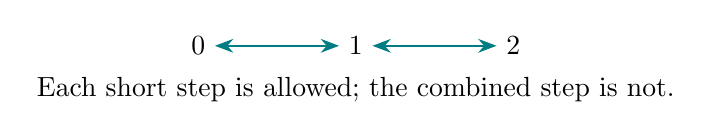
\begin{tikzpicture}[>=Stealth,x=2cm]
\node (a) at (0,0) {$0$}; \node (b) at (1,0) {$1$}; \node (c) at (2,0) {$2$};
\draw[<->,thick,ProofTeal] (a)--(b);
\draw[<->,thick,ProofTeal] (b)--(c);
\node at (1,-.55) {Each short step is allowed; the combined step is not.};
\end{tikzpicture}
\end{center}
\sourcecredit{Example 10.1.3; new counterexample choices and diagram}
\end{frame}

% Source: Example 10.1.4, exactly the three directed edges in the source relation.
\begin{frame}{A finite directed cycle is antisymmetric}
\begin{columns}[T]
\begin{column}{.44\textwidth}
Let $x\prec y$ mean ``$x$ loses to $y$'' for rock, paper, and scissors.
The diagram lists all related pairs.
\begin{center}
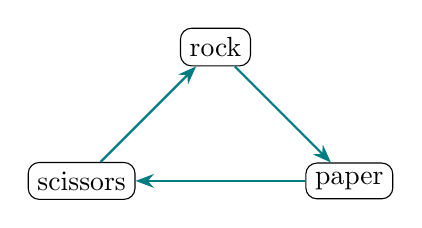
\begin{tikzpicture}[>=Stealth]
\node[draw,rounded corners] (r) at (0,1.7) {rock};
\node[draw,rounded corners] (p) at (1.7,0) {paper};
\node[draw,rounded corners] (s) at (-1.7,0) {scissors};
\draw[->,thick,ProofTeal] (r)--(p);
\draw[->,thick,ProofTeal] (p)--(s);
\draw[->,thick,ProofTeal] (s)--(r);
\end{tikzpicture}
\end{center}
\end{column}
\begin{column}{.53\textwidth}
\begin{itemize}
\item Not reflexive: there is no loop at rock.
\item Not symmetric: rock $\prec$ paper, but paper $\not\prec$ rock.
\item Antisymmetric: no pair has arrows in both directions, so its two-premise implication always holds.
\item Not transitive: rock $\prec$ paper and paper $\prec$ scissors, but rock $\not\prec$ scissors.
\end{itemize}
\end{column}
\end{columns}
\sourcecredit{Example 10.1.4; original drawing}
\end{frame}

% Source: Two exercises from 10.1.5, subset and coordinatewise order.
\begin{frame}{Practice 10.1: Prove or refute each property}
For each relation, decide whether it is reflexive, symmetric, antisymmetric, and transitive.
\begin{enumerate}
\item On $\mathcal P(\N)$, define $U\sim V$ by $U\subseteq V$.
Your variables are now sets of natural numbers.
\item On $\R^2$, define
\[
 (x_1,y_1)\preceq(x_2,y_2)
 \quad\Longleftrightarrow\quad
 x_1\le x_2\ \land\ y_1\le y_2.
\]
Your variables are now ordered pairs of real numbers.
\end{enumerate}
Each positive answer needs a universal proof; each negative answer needs a suitable counterexample.
\sourcecredit{Exercises 10.1.5}
\end{frame}

% Source: New solutions for the subset exercise in 10.1.5.
\begin{frame}{Practice 10.1: Inclusion on sets of natural numbers}
\begin{itemize}
\item \textbf{Reflexive.} $U\subseteq U$: an arbitrary element of $U$ already belongs to $U$.
\item \textbf{Not symmetric.} $\emptyset\subseteq\{0\}$, but $\{0\}\not\subseteq\emptyset$
because $0\notin\emptyset$.
\item \textbf{Antisymmetric.} If $U\subseteq V$ and $V\subseteq U$, then for every $n\in\N$,
$n\in U\iff n\in V$. Set extensionality gives $U=V$.
\item \textbf{Transitive.} If $U\subseteq V$ and $V\subseteq W$, take $n\in U$.
The first inclusion gives $n\in V$, and the second gives $n\in W$.
Thus $U\subseteq W$.
\end{itemize}
The chapter on sets already supplied the proof of antisymmetry; here we recognize its role as a relation property.
\sourcecredit{Exercises 10.1.5; set extensionality from Section 9.1}
\end{frame}

% Source: New solutions for the coordinatewise-order exercise in 10.1.5.
\begin{frame}{Practice 10.1: Compare the coordinates separately}
For $\preceq$ on $\R^2$:
\begin{itemize}
\item \textbf{Reflexive.} $x\le x$ and $y\le y$, so $(x,y)\preceq(x,y)$.
\item \textbf{Not symmetric.} $(0,0)\preceq(1,1)$, but the reverse would require $1\le0$.
\item \textbf{Antisymmetric.} Relations in both directions give
$x_1\le x_2\le x_1$ and $y_1\le y_2\le y_1$.
Thus $x_1=x_2$ and $y_1=y_2$, so the pairs are equal.
\item \textbf{Transitive.} From $(x_1,y_1)\preceq(x_2,y_2)$ and
$(x_2,y_2)\preceq(x_3,y_3)$, obtain
$x_1\le x_2\le x_3$ and $y_1\le y_2\le y_3$.
Hence $(x_1,y_1)\preceq(x_3,y_3)$.
\end{itemize}
Not every two points are comparable: $(0,1)$ and $(1,0)$ provide an example.
\sourcecredit{Exercises 10.1.5}
\end{frame}

\section{10.2 Equivalence relations}
% Source: Definition and Example 10.2.1. All n in Z, including zero, are retained.
\begin{frame}{10.2: Equivalence relations formalize a notion of sameness}
\begin{block}{Definition}
A relation is an \emph{equivalence relation} if it is reflexive, symmetric, and transitive.
\end{block}
Fix any $n\in\Z$. On $\Z$, let $x\sim y$ mean $x\equiv y\pmod n$,
equivalently $y-x=nk$ for some $k\in\Z$.
\begin{itemize}
\item \textbf{Reflexive:} $x-x=n\cdot0$.
\item \textbf{Symmetric:} if $y-x=nk$, then $x-y=n(-k)$.
\item \textbf{Transitive:} if $y-x=nk$ and $z-y=nl$, then
$z-x=(z-y)+(y-x)=n(l+k)$.
\end{itemize}
The argument needs no positivity assumption on $n$. When $n=0$, the relation is equality,
because $0\mid(y-x)$ holds exactly when $y-x=0$.
\sourcecredit{Example 10.2.1}
\end{frame}

% Source: Examples 10.2.1 and 10.2.3. Original labelled class diagram.
\begin{frame}{Equivalence classes collect the elements related to one element}
For a relation on $X$ and $a\in X$, define
\[
 [a]=\{b:X\mid a\sim b\}.
\]
For congruence modulo $3$ on $\Z$, there are three classes:
\begin{center}

\begin{tikzpicture}[x=1cm,y=1cm]
\node[draw=ProofTeal,fill=ProofTeal!10,rounded corners,text width=10cm,align=center] at (0,1.4)
 {$[0]=\{\ldots,-6,-3,0,3,6,\ldots\}$};
\node[draw=ProofNavy,fill=ProofNavy!7,rounded corners,text width=10cm,align=center] at (0,.55)
 {$[1]=\{\ldots,-5,-2,1,4,7,\ldots\}$};
\node[draw=ProofTeal,fill=ProofTeal!20,rounded corners,text width=10cm,align=center] at (0,-.3)
 {$[2]=\{\ldots,-4,-1,2,5,8,\ldots\}$};
\end{tikzpicture}
\end{center}
Two integers are related exactly when they lie in the same row.
Every integer is in its own class because the relation is reflexive.
\sourcecredit{Examples 10.2.1 and 10.2.3}
\end{frame}

% Source: Example 10.2.2, with the symmetry conclusion corrected from y~z to y~x.
\begin{frame}{Equal squares give another equivalence relation}
On $\Z$, define $a\sim b$ by $a^2=b^2$.
\begin{itemize}
\item \textbf{Reflexive:} $a^2=a^2$ for every integer $a$.
\item \textbf{Symmetric:} $a^2=b^2$ implies $b^2=a^2$.
\item \textbf{Transitive:} $a^2=b^2$ and $b^2=c^2$ imply $a^2=c^2$.
\end{itemize}
What are its classes? Since
\[
 a^2=b^2\quad\Longleftrightarrow\quad(a-b)(a+b)=0,
\]
we have $b=a$ or $b=-a$. Thus $[0]=\{0\}$ and $[a]=\{a,-a\}$ for $a\ne0$.
\medskip

This relation is not antisymmetric: $1\sim-1$ and $-1\sim1$, yet $1\ne-1$.
Equivalence does not require antisymmetry.
\sourcecredit{Example 10.2.2}
\end{frame}

% Source: Example 10.2.2, ASCII statement and direct equality methods.
\begin{frame}[fragile]{Lean: Reuse the corresponding property of equality}
\begin{lstlisting}
def sameSquare (x y : Int) : Prop := x ^ 2 = y ^ 2

example : Reflexive sameSquare := by
  intro x
  rfl

example : Symmetric sameSquare := by
  intro x y h
  exact h.symm

example : Transitive sameSquare := by
  intro x y z hxy hyz
  exact hxy.trans hyz
\end{lstlisting}
Once the relation unfolds, reflexivity, symmetry, and transitivity become the corresponding
facts about equality of squares.
\sourcecredit{Example 10.2.2; textbook-environment demonstration}
\end{frame}

% Source: Both theorems in Example 10.2.3. The first requires only symmetry and transitivity.
\begin{frame}{Related elements have equal classes}
\begin{block}{Theorem with its precise hypotheses}
If $\sim$ is symmetric and transitive on $X$, and $a_1\sim a_2$,
then $[a_1]=[a_2]$.
\end{block}
Fix $b\in X$. We prove $a_1\sim b\iff a_2\sim b$.
\begin{itemize}
\item If $a_1\sim b$, symmetry gives $a_2\sim a_1$.
Transitivity along $a_2\sim a_1\sim b$ gives $a_2\sim b$.
\item If $a_2\sim b$, transitivity along $a_1\sim a_2\sim b$ gives $a_1\sim b$.
\end{itemize}
Extensionality now gives the equality of sets. Reflexivity was not needed for this theorem.
\medskip

Separately, if the relation is reflexive, then $a\in[a]$ for every $a$,
because that membership statement is exactly $a\sim a$.
\sourcecredit{Example 10.2.3}
\end{frame}

% Source: The class theorems of 10.2.3; the partition corollary is an original derivation.
\begin{frame}{Why equivalence classes form a partition}
Assume $\sim$ is an equivalence relation on $X$.
\begin{itemize}
\item \textbf{The classes cover $X$.} Every $a\in X$ belongs to $[a]$ by reflexivity.
\item \textbf{Overlapping classes are equal.} Suppose $c\in[a]\cap[b]$.
Then $a\sim c$ and $b\sim c$. Symmetry gives $c\sim b$, and transitivity gives $a\sim b$.
The preceding theorem yields $[a]=[b]$.
\end{itemize}
Thus any two classes are either equal or disjoint. The distinct classes split $X$
into nonempty, nonoverlapping pieces: a \emph{partition}.
\medskip

For equality on $\Z$, each class is a singleton: $[a]=\{a\}$.
For equal squares on $\Z$, most classes contain two integers instead.
\sourcecredit{Example 10.2.3 and Example 10.2.4; partition corollary derived here}
\end{frame}

% Source: Example 10.2.5; natural second coordinates and integer products are preserved.
\begin{frame}{Pairs can represent the same rational value}
On $\Z\times\N$, define
\[
 (a,b)\sim(c,d)\quad\Longleftrightarrow\quad a(d+1)=c(b+1).
\]
The products are taken in $\Z$; the natural numbers $b,d$ are viewed as integers.
Since $b+1,d+1>0$, this condition means
\[
 \frac{a}{b+1}=\frac{c}{d+1}\qquad\text{in }\Q.
\]
For example, $(1,1)\sim(2,3)$ because $1\cdot4=2\cdot2$.
\begin{itemize}
\item Reflexivity follows from $a(b+1)=a(b+1)$.
\item Symmetry follows by reversing the equality $a(d+1)=c(b+1)$.
\end{itemize}
Transitivity requires a calculation and cancellation of a nonzero factor.
\sourcecredit{Example 10.2.5}
\end{frame}

% Source: Transitivity proof in Example 10.2.5.
\begin{frame}{Transitivity for the pair representation}
Assume $(a,b)\sim(c,d)$ and $(c,d)\sim(e,f)$.
Set $B=b+1$, $D=d+1$, and $F=f+1$, as integers. Then
\[
 aD=cB,\qquad cF=eD,\qquad D>0.
\]
We want $aF=eB$. First calculate
\[
\begin{aligned}
 D(aF)&=(aD)F\\
      &=(cB)F\\
      &=(cF)B\\
      &=(eD)B\\
      &=D(eB).
\end{aligned}
\]
Since $D\ne0$, cancellation gives $aF=eB$, as required.
In the book's Lean proof, \texttt{ring} rearranges products, \texttt{rw} uses the hypotheses,
and \texttt{cancel D at this} performs the final cancellation.
\sourcecredit{Example 10.2.5}
\end{frame}

% Source: Example 10.2.6, relation on level-0 types.
\begin{frame}{Having a bijection is an equivalence relation on types}
For level-0 types $X,Y$ (Lean: \texttt{Type}), define
\[
 X\sim Y\quad\Longleftrightarrow\quad
 \text{there exists a bijective function }f:X\to Y.
\]
\begin{itemize}
\item \textbf{Reflexive.} The identity $\operatorname{id}_X:X\to X$ is its own inverse,
so it is bijective.
\item \textbf{Symmetric.} If $f:X\to Y$ is bijective, it has an inverse $g:Y\to X$.
The two inverse identities also show that $f$ is an inverse of $g$; hence $g$ is bijective.
\item \textbf{Transitive.} Given bijections $f:X\to Y$ and $g:Y\to Z$,
their composition $g\circ f:X\to Z$ is injective and surjective by the composition proofs in Chapter 8.
\end{itemize}
The relation records that two types can be matched exactly, even when their elements look different.
\sourcecredit{Example 10.2.6; Section 8.3}
\end{frame}

% Source: First two exercises in 10.2.7.
\begin{frame}{Practice 10.2: Prove equivalence and describe the classes}
\begin{enumerate}
\item On $\Z$, define $a\sim b$ when there are positive integers $m,n$ such that
$am=bn$. Prove this is an equivalence relation and determine its classes.
\item On $\N^2$, define
\[
 (a,b)\approx(c,d)\quad\Longleftrightarrow\quad a+d=b+c.
\]
Prove this is an equivalence relation. Describe its classes using the integer difference $a-b$.
\end{enumerate}
In the first problem, positivity is part of the definition.
In the second, interpret differences in $\Z$, not as truncated subtraction in $\N$.
\sourcecredit{Exercises 10.2.7}
\end{frame}

% Source: New solution to the first exercise in 10.2.7.
\begin{frame}{Practice 10.2: Positive multiples and the three sign classes}
\begin{itemize}
\item \textbf{Reflexive:} use $m=n=1$.
\item \textbf{Symmetric:} if $am=bn$ with $m,n>0$, reverse the equation and swap the witnesses.
\item \textbf{Transitive:} suppose $am=bn$ and $bp=cq$, with all four witnesses positive.
Then $a(mp)=b(np)=c(qn)$; both $mp$ and $qn$ are positive.
\end{itemize}
There are exactly three classes: the positive integers, $\{0\}$, and the negative integers.
\begin{itemize}
\item Positive multiplication preserves sign, so related integers have the same sign,
including being zero together.
\item If $a,b>0$, choose $m=b,n=a$. If $a,b<0$, choose $m=-b,n=-a$.
These positive witnesses show that any two integers in either sign group are related.
\end{itemize}
\sourcecredit{Exercises 10.2.7, first problem}
\end{frame}

% Source: New solution to the second exercise in 10.2.7; no Nat-subtraction ambiguity.
\begin{frame}{Practice 10.2: Equal differences of natural-number pairs}
For $(a,b),(c,d)\in\N^2$, the equation $a+d=b+c$ is equivalent to
\[
 a-b=c-d\qquad\text{when evaluated in }\Z.
\]
\begin{itemize}
\item Reflexivity is $a+b=b+a$.
\item Symmetry follows by reversing the equality of integer differences.
\item Transitivity follows from $a-b=c-d$ and $c-d=e-f$, which give $a-b=e-f$,
and hence $a+f=b+e$.
\end{itemize}
For each $k\in\Z$, one class is
\[
 C_k=\{(a,b)\in\N^2\mid a-b=k\text{ in }\Z\}.
\]
Each class is nonempty: use $(k,0)$ if $k\ge0$, or $(0,-k)$ if $k<0$.
Geometrically these classes lie on parallel diagonals in the natural-number grid.
\sourcecredit{Exercises 10.2.7, second problem}
\end{frame}

% Source: Review synthesized from Examples 10.1.1--10.1.4 and Section 10.2.
\begin{frame}{Chapter 10 review: Classify the relation before using it}
\begin{center}
\begin{tabular}{lcccc}
\toprule
Relation and ambient type & Refl. & Symm. & Antisymm. & Trans.\\\midrule
$=$ on $\R$ & yes & yes & yes & yes\\
$\mid$ on $\N$ & yes & no & yes & yes\\
$(x-y)^2\le1$ on $\R$ & yes & yes & no & no\\
Loses-to on three hands & no & no & yes & no\\
$a^2=b^2$ on $\Z$ & yes & yes & no & yes\\
\bottomrule
\end{tabular}
\end{center}
An equivalence relation needs the first, second, and fourth properties.
Its equivalence classes cover the type, and overlapping classes are equal.
\medskip

\textbf{Exit check.} If an equivalence relation is also antisymmetric, prove it is equality:
$a\sim b$ gives $b\sim a$ by symmetry, hence $a=b$; reflexivity gives the converse.
\sourcecredit{Examples 10.1.1--10.1.4; Section 10.2}
\end{frame}

% Source and adaptation statement for the chapter.
\begin{frame}{Reading and code context}
Heather Macbeth, \emph{The Mechanics of Proof}, Chapter 10:
\begin{itemize}
\item 10.1 Reflexive, symmetric, antisymmetric, transitive
\item 10.2 Equivalence relations
\end{itemize}
\url{https://hrmacbeth.github.io/math2001/10_Relations.html}
\medskip

These notes include original diagrams, worked practice solutions, and the derived partition corollary.
Lean examples use the textbook's teaching environment; its relation-property names are
\texttt{Reflexive}, \texttt{Symmetric}, \texttt{AntiSymmetric}, and \texttt{Transitive}.
The spelling of antisymmetry follows that source environment.
\end{frame}
\end{document}
